\subsubsection{The Tosi et al.~benchmarks}
\label{sec:benchmark-tosii}

\textit{This section was contributed by Anne Glerum.}

This section discusses the viscoplastic thermal convection benchmarks described by Tosi et al.~\cite{T15}.  The five benchmarks extend those of Blankenbach et al.~\cite{BBC89} with temperature-, pressure- and strain rate-dependent rheology. As the \aspect{} results are published in the original paper, we limit ourselves to a brief description of the setup and results of the first 2 benchmark cases.

All five benchmarks solve for Boussinesq convection in a box of $1 \times 1$ dimensions with free slip boundary conditions. The initial temperature distribution considers a linear depth profile with a slight perturbation to start convection. Top and bottom boundaries are set to a fixed temperature value. The parameters shared between the benchmark cases can be found in \url{benchmarks/tosi_et_al_2015_gcubed/Tosi_base.prm}. The other input files describe the variations on this base model, which pertain to the rheological description. The specific rheologies used are implemented in \url{benchmarks/tosi_et_al_2015_gcubed/tosi.cc} and describe a linear and a plastic component of the viscosity:
\begin{align}
  \eta_\text{linear}(T,z) &= \exp(-\ln(\eta_T) T + \ln(\eta_Z) z)
  \label{eq:tosi-benchmark-lin-visc} \\
  \eta_\text{plastic}(\dot\epsilon) &= \eta^\ast + \frac{\sigma_y}{\sqrt{\dot\epsilon:\dot\epsilon}}
  \label{eq:tosi-benchmark-plast-visc}
\end{align}
where $\eta^\ast$ is the constant effective viscosity at high stresses and $\sigma_y$ the yield stress.

\paragraph{Case 1: Temperature-dependent convection.}
\label{sec:benchmark-tosi-case-1}

The first benchmark considers a viscosity that only depends on temperature (Eq. \eqref{eq:tosi-benchmark-lin-visc}, with $\gamma_Z=0$). When run to steady-state, this produces one convection cell with a high viscosity, stagnant lid insulating the fluid below (see Fig. 1 of \cite{T15}). In \cite{T15}, results of different codes are compared by looking at the average temperature, the Nusselt number at the top and bottom of the domain, the RMS velocity at the top boundary and in the whole domain, and the maximum velocity at the surface. These quantities can be queried by using several of the \aspect{} postprocessors, but the additional postprocessor in \url{benchmarks/tosi_et_al_2015_gcubed/tosi.cc} is needed to compute the average rate of work done against gravity, the average rate of viscous dissipation, and the error between them. Differences between these diagnostic quantities of the 11 codes that participated in the benchmark effort are smaller than 5\% for their preferred mesh resolution.

\paragraph{Case 2: Viscoplastic convection.}
\label{sec:benchmark-tosi-case-2}
Case 2 includes a strain rate-dependent component in the viscosity, which is harmonically averaged with the linear component (see also the code snippet below):

\begin{equation}
  \eta(T,\epsilon,z) = 2 \left(\frac{1}{\eta_\text{linear}}+\frac{1}{\eta_\text{plastic}}\right)^{-1}
  \label{eq:tosi-benchmark-ave-visc}
\end{equation}

\lstinputlisting[language=prmfile]{cookbooks/benchmarks/tosi_et_al_2015_gcubed/doc/tosi_benchmark_2.prm.out}

This rheology leads to mobile-lid convection, with the descending cold lid cooling the cell's interior (Fig. 2 of \cite{T15}).

By changing the input parameters shown in the code snippet, we obtain the other benchmark cases.
Case 3 includes a depth-dependent component for the viscosity, but no strain rate-dependence, i.e. it uses Eq. \eqref{eq:tosi-benchmark-lin-visc}. Case 4 considers a full temperature-, depth- and strain rate-dependent viscosity, while in case 5 the yield stress is varied to investigate the transitions from mobile-lid to periodic to stagnant-lid convection regimes.
The input files referenced above implement these specific cases. As mentioned before, the \aspect{} results are presented in \cite{T15} together with the results of several other finite element, finite volume, and spectral codes. Figure~\ref{fig:tosi-benchmark-results} shows one example of the resolved temperature and viscosity fields for case 1.

\begin{figure}
  \begin{center}
    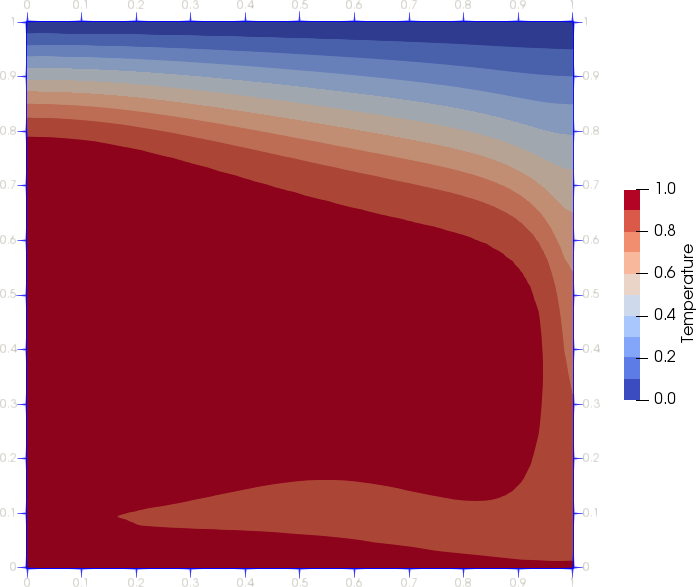
\includegraphics[width=0.31\textwidth]{cookbooks/benchmarks/tosi_et_al_2015_gcubed/doc/Case1_6_T.png}
    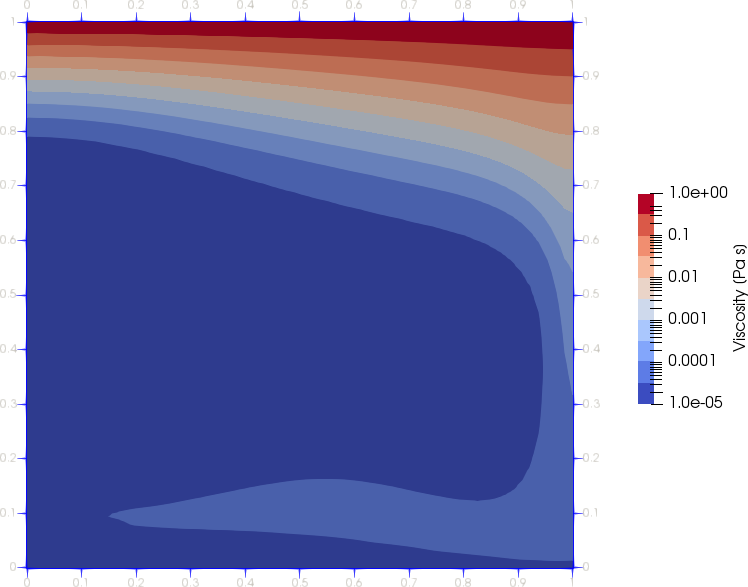
\includegraphics[width=0.31\textwidth]{cookbooks/benchmarks/tosi_et_al_2015_gcubed/doc/Case1_6_visc.png}
    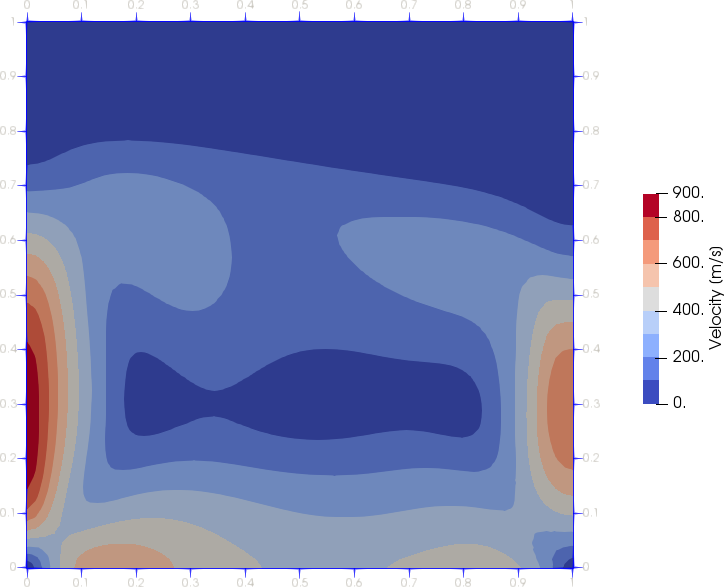
\includegraphics[width=0.31\textwidth]{cookbooks/benchmarks/tosi_et_al_2015_gcubed/doc/Case1_6_vel.png}
  \end{center}
  \caption{\it Temperature and viscosity field in steady-state for case 1 of \cite{T15}.}
  \label{fig:tosi-benchmark-results}
\end{figure}

